\chapter{Online Algorithms for Continuous POMDPs}

\section{Background}

Although the research surveyed in \cref{sec:solutions} has yielded effective solution techniques for many classes of POMDPs, there remains a need for simple, general purpose online solvers that can handle continuous spaces, especially continuous observation spaces.
This chapter addresses that need.

Many previous methods can easily handle continuous state spaces \cite{goldhoorn2014continuous}, but they must be modified to extend to domains with continuous action or observation spaces.
Though DESPOT has demonstrated effectiveness on some large problems, since it uses unweighted particle beliefs in its search tree, it struggles with continuous information gathering problems as will be shown in \cref{sec:experiments}.
ABT has been extended to use generalized pattern search for selecting locally optimal continuous actions, an approach which is especially effective in problems where high precision is important \cite{seiler2015online}, but also uses unweighted particle beliefs.
Continuous observation Monte Carlo tree search (COMCTS) constructs observation classification trees to automatically partition the observation space in a POMCP-like approach, however it did not perform much better than a Monte Carlo rollout approach in experiments \cite{pas2012simulation}.

The algorithms discussed in this chapter are derivatives of the partially observable Monte Carlo planning algorithm (POMCP), which is based on MCTS (\cref{sec:mcts}).
A conceptually straightforward way to solve a POMDP using MCTS is to apply it to the corresponding belief MDP.
Indeed, many tree search techniques have been applied to POMDP problems in this way \cite{ross2008online}.
However, when the Bayesian belief update is used, this approach is computationally expensive.
POMCP and its successors, DESPOT and ABT, can tackle problems many times larger than their predecessors because they use state trajectory simulations, rather than full belief trajectories, to build the tree.

Each of the nodes in a POMCP tree corresponds to a history proceeding from the root belief and terminating with an action or observation.
In the search phase of POMCP tree construction, state trajectories are simulated through this tree.
At each action node, the rewards from the simulations that pass through the node are used to estimate the $Q$ function.
This simple approach has been shown to work well for large discrete problems \cite{silver2010pomcp}.
However, when the action or observation space is continuous, the tree degenerates and does not extend beyond a single layer of nodes because each new simulation produces a new branch.

\section{Structure and Notation}

The three algorithms in this section share a common structure.
For all algorithms, the entry point for the decision making process is the \textproc{Plan} procedure, which takes the current belief, $b$, as an input (\textproc{Plan} differs slightly for PFT-DPW in \cref{alg:pft}).
The algorithms also share the same \textproc{ActionProgWiden} function to control progressive widening of the action space.
These components are listed in Listing \ref{alg:common}.
The difference between the algorithms is in the \textproc{Simulate} function.

The following variables are used in the listings and text:
$h$ represents a history $(b, a_1, o_1, \dots a_k, o_k)$, and $ha$ and $hao$ are shorthand for histories with $a$ and $(a,o)$ appended to the end, respectively;
$d$ is the depth to explore, with $d_\text{max}$ the maximum depth;
$C$ is a list of the children of a node (along with the reward in the case of PFT-DPW);
$N$ is a count of the number of visits; and $M$ is a count of the number of times that a history has been generated by the model.
The list of states associated with a node is denoted $B$, and $W$ is a list of weights corresponding to those states.
Finally, $Q(ha)$ is an estimate of the value of taking action $a$ after observing history $h$.
$C$, $N$, $M$, $B$, $W$, and $Q$ are all implicitly initialized to \num{0} or $\emptyset$.
The \textproc{Rollout} procedure, runs a simulation with a default rollout policy, which can be based on the history or fully observed state for $d$ steps and returns the discounted reward.

% TODO algorithm vs listing numbering
\begin{algorithm}[t]
    \floatname{algorithm}{Listing}
    \caption{Common procedures} \label{alg:common}
    \begin{algorithmic}[1]
        \Procedure{Plan}{$b$}
            \For{$i \in 1:n$}
                \State $s \gets \text{sample from }b$
                \State $\Call{Simulate}{s, b, d_\text{max}}$
            \EndFor
            \State $\textbf{return } \underset{a}{\argmax}\, Q(ba)$
        \EndProcedure

        \Procedure {ActionProgWiden}{$h$}
            \If{$|C(h)| \leq k_a N(h)^{\alpha_a}$}
                \State $a \gets \Call{NextAction}{h}$
                \State $C(h) \gets C(h) \cup \{a\}$
            \EndIf
            \State $\textbf{return } \underset{a \in C(h)}{\argmax}\, Q(ha) + c \sqrt{\frac{\log N(h)}{N(ha)}}$
        \EndProcedure

    \end{algorithmic}
\end{algorithm}


\section{POMCP-DPW}

The first algorithm that we consider is POMCP with double progressive widening (POMCP-DPW).
In this algorithm, listed in \cref{alg:pomcpdpw}, the number of new children sampled from any node in the tree is limited by DPW using the parameters $k_a$, $\alpha_a$, $k_o$, and $\alpha_o$.
In the case where the simulated observation is rejected (line~\ref{lin:notnew}), the tree search is continued with an observation selected in proportion to the number of times, $M$, it has been previously simulated (line~\ref{lin:selecto}) and a state is sampled from the associated belief (line~\ref{lin:samples}).

\setcounter{algorithm}{0}
\begin{algorithm}
    \caption{POMCP-DPW} \label{alg:pomcpdpw}
    \begin{algorithmic}[1]
        \Procedure {Simulate}{$s$, $h$, $d$}        
            \If{$d = 0$}
                \State \textbf{return} $0$
            \EndIf
            \State $a \gets \Call{ActionProgWiden}{h}$
            \If{$|C(ha)| \leq k_o N(ha)^{\alpha_o}$}
                \State $s',o,r \gets G(s,a)$
                \State $C(ha) \gets C(ha) \cup \{o\}$
                \State $M(hao) \gets M(hao) + 1$
                \State $\text{append } s' \text{ to } B(hao)$ \label{lin:insertion}
                \If{$M(hao) = 1$}
                    \State $total \gets r + \gamma \Call{Rollout}{s', hao, d-1}$
                \Else
                    \State $total \gets r + \gamma \Call{Simulate}{s', hao, d-1}$
                \EndIf
            \Else \label{lin:notnew}
                \State $o \gets \text{select } o \in C(ha) \text{ w.p. } \frac{M(hao)}{\sum_{o} M(hao)}$ \label{lin:selecto}
                \State $s' \gets \text{select } s' \in B(hao) \text{ w.p. } \frac{1}{|B(hao)|}$ \label{lin:samples}
                \State $r \gets R(s,a,s')$
                \State $total \gets r + \gamma \Call{Simulate}{s', hao, d-1}$
            \EndIf
            \State $N(h) \gets N(h)+1$
            \State $N(ha) \gets N(ha)+1$
            \State $Q(ha) \gets Q(ha) + \frac{total - Q(ha)}{N(ha)}$
            \State \textbf{return} $total$
        \EndProcedure
    \end{algorithmic}
\end{algorithm}

This algorithm obtained remarkably good solutions for a very large autonomous freeway driving POMDP with multiple vehicles (up to 40 continuous fully observable state dimensions and 72 continuous correlated partially observable state dimensions) \cite{sunberg2017value}.
To our knowledge, that is the first work applying progressive widening to POMCP, and it does not contain a detailed description of the algorithm or any theoretical or experimental analysis other than the driving application.

This algorithm may converge to the optimal solution for POMDPs with discrete observation spaces; however, on continuous observation spaces, POMCP-DPW is suboptimal.
In particular, it finds a QMDP policy, that is, the solution under the assumption that the problem becomes fully observable after one time step \cite{littman1995learning,kochenderfer2015decision}.
In fact, for a modified version of POMCP-DPW, it is easy to prove analytically that it will converge to such a policy.
This is expressed formally in Theorem~\ref{thm:qmdp} below.
A complete description of the modified algorithm and problem requirements including the definitions of polynomial exploration, the regularity hypothesis for the problem, and exponentially sure convergence are given in \cref{sec:proof}.

\begin{definition}[QMDP value]
    Let $Q_\text{MDP}(s,a)$ be the optimal state-action value function assuming full observability starting by taking action $a$ in state $s$. The \emph{QMDP value} at belief $b$, $Q_\text{MDP}(b,a)$, is the expected value of $Q_\text{MDP}(s,a)$ when $s$ is distributed according to $b$.
\end{definition}

% \begin{theorem}[Modified POMCP-DPW convergence to QMDP] \label{thm:qmdp}
\begin{restatable}[Modified POMCP-DPW convergence to QMDP]{theorem}{qmdp}
    \label{thm:qmdp}
If a bounded-horizon POMDP meets the following conditions: 1) the state and observation spaces are continuous with a finite observation probability density function, and 2) the regularity hypothesis is met, then modified POMCP-DPW will produce a value function estimate, $\hat{Q}$, that converges to the QMDP value for the problem.
Specifically, there exists a constant $C>0$, such that after $n$ iterations,
\begin{equation*}
    \left| \hat{Q}(b,a) - Q_\text{MDP}(b,a) \right| \leq \frac{C}{n^{1/(10d_{\max}-7)}}
\end{equation*}
exponentially surely in $n$, for every action $a$.
\end{restatable}
% \end{theorem}

A proof of this theorem that leverages work by \citet{auger2013continuous} is given in \cref{sec:proof}, but we provide a brief justification here.
The key is that belief nodes will contain only a single state particle (see \cref{fig:treecomp}).
This is because, since the observation space is continuous with a finite density function, the generative model will (with probability one) produce a unique observation $o$ each time it is queried.
Thus, for every generated history $h$, only one state will ever be inserted into $B(h)$ (line~\ref{lin:insertion}, \cref{alg:pomcpdpw}), and therefore $h$ is merely an alias for that state. 
Since each belief node corresponds to a state, the solver is actually solving the fully observable MDP at every node except the root node, leading to a QMDP solution.

As a result of \cref{thm:qmdp}, the action chosen by modified POMCP-DPW will match a QMDP policy (a policy of actions that maximize the QMDP value) with high precision exponentially surely (see Corollary 1 of \citet{auger2013continuous}).
For many problems this is a very useful solution,\footnote{Indeed, a useful online QMDP tree search algorithm could be created by deliberately constructing a tree with a single root belief node and fully observable state nodes below it.} but since it neglects the value of information, a QMDP policy is suboptimal for problems where information gathering is important \cite{littman1995learning,kochenderfer2015decision}.
% This phenomenon is demonstrated in simulation in \cref{sec:lightdark}.

Although \cref{thm:qmdp} is only theoretically applicable to the modified version of POMCP-DPW, it helps explain the behavior of other solvers.
Modified POMCP-DPW, POMCP-DPW, DESPOT, and ABT all share the characteristic that a belief node can only contain two states if they generated exactly the same observation.
Since this is an event with zero probability for a continuous observation space, these solvers exhibit suboptimal, often QMDP-like, behavior.
The experiments in \cref{sec:experiments} show this for POMCP-DPW and DESPOT, and this is presumably the case for ABT as well.


\begin{figure}[htpb]
    \centering
    \begin{subfigure}[b]{0.45\columnwidth}
        \centering
        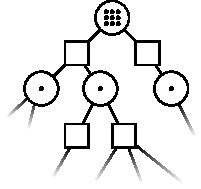
\includegraphics[width=\textwidth]{media/dpw_tree.pdf}
        \caption{POMCP-DPW Tree}
    \end{subfigure}
    \begin{subfigure}[b]{0.45\columnwidth}
        \centering
        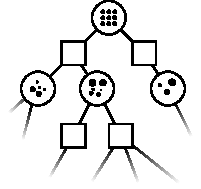
\includegraphics[width=\textwidth]{media/pomcpow_tree.pdf}
        \caption{POMCPOW Tree}
    \end{subfigure}
    \caption{Tree Structure Comparison. Each square is an action node, and each unfilled circle is an observation node. Each black dot corresponds to a state particle with the size representing its weight. In continuous observation spaces, the beliefs in a POMCP-DPW tree degenerate to a single particle, while POMCPOW maintains weighted particle mixture beliefs.}
    \label{fig:treecomp}
\end{figure}

\section{PFT-DPW}

Another algorithm that one might consider for solving continuous POMDPs online is MCTS-DPW on the equivalent belief MDP.
Since the Bayesian belief update is usually computationally intractable, a particle filter is used.
This new approach will be referred to as particle filter trees with double progressive widening (PFT-DPW).
It is shown in \cref{alg:pft}, where $G_\text{PF($m$)}(b,a)$ is a particle filter belief update performed with a simulated observation and $m$ state particles which approximates the belief MDP generative model.
The authors are not aware of any mention of this algorithm in prior literature, but it is very likely that MCTS with particle filters has been used before without double progressive widening under another name.

PFT-DPW is fundamentally different from POMCP and POMCPOW because it relies on simulating approximate belief trajectories instead of state trajectories.
This distinction also allows it to be applied to problems where the reward is a function of the belief rather than the state such as pure information-gathering problems \cite{dressel2017efficient,araya2010pomdp}.

The primary shortcoming of this algorithm is that the number of particles in the filter, $m$, must be chosen a-priori and is static throughout the tree.
Each time a new belief node is created, an $\mathcal{O}(m)$ particle filter update is performed.
If $m$ is too small, the beliefs may miss important states, but if $m$ is too large, constructing the tree is expensive.
Fortunately, the experiments in \cref{sec:experiments} show that it is often easy to choose $m$ in practice; for all the problems we studied, a value of $m=20$ resulted in good performance.


\begin{algorithm}
    \caption{PFT-DPW} \label{alg:pft}
    \begin{algorithmic}[1]
        \Procedure{Plan}{$b$}
            \For{$i \in 1:n$}
                \State $\Call{Simulate}{b, d_\text{max}}$
            \EndFor
            \State $\textbf{return } \underset{a}{\argmax}\, Q(ba)$
        \EndProcedure
        \Procedure {Simulate}{$b$, $d$}        
            \If{$d = 0$}
                \State \textbf{return} $0$
            \EndIf
            \State $a \gets \Call{ActionProgWiden}{b}$
            \If{$|C(ba)| \leq k_o N(ba)^{\alpha_o}$}
                \State $b',r \gets G_\text{PF($m$)}(b,a)$
                \State $C(ba) \gets C(ba) \cup \{(b',r)\}$
                \State $total \gets r + \gamma \Call{Rollout}{b', d-1}$
            \Else
                \State $b', r \gets \text{sample uniformly from } C(ba)$
                \State $total \gets r + \gamma \Call{Simulate}{b', d-1}$
            \EndIf
            \State $N(b) \gets N(b)+1$
            \State $N(ba) \gets N(ba)+1$
            \State $Q(ba) \gets Q(ba) + \frac{total - Q(ba)}{N(ba)}$
            \State \textbf{return} $total$
        \EndProcedure
    \end{algorithmic}
\end{algorithm}

\subsection{POMCPOW} \label{sec:pomcpow}

\begin{algorithm}[t]
    \caption{POMCPOW} \label{alg:pomcpow}
    \begin{algorithmic}[1]
        \Procedure {Simulate}{$s$, $h$, $d$}        
            \If{$d = 0$}
                \State \textbf{return} $0$
            \EndIf
            \State $a \gets \Call{ActionProgWiden}{h}$
            \State $s',o,r \gets G(s,a)$
            \If{$|C(ha)| \leq k_o N(ha)^{\alpha_o}$}
                \State $M(hao) \gets M(hao) + 1$
            \Else
                \State $o \gets \text{select } o \in C(ha) \text{ w.p. } \frac{M(hao)}{\sum_{o} M(hao)}$
            \EndIf
            \State $\text{append } s' \text{ to } B(hao)$ \label{lin:insert}
            \State $\text{append } \odist(o \mid s, a, s') \text{ to } W(hao)$ \label{lin:weight}
            \If{$o \notin C(ha)$} \Comment{new node}
                \State $C(ha) \gets C(ha) \cup \{o\}$
                \State $total \gets r + \gamma \Call{Rollout}{s', hao, d-1}$
            \Else
                \State $s' \gets \text{select } B(hao)[i] \text{ w.p. } \frac{W(hao)[i]}{\sum_{j=1}^m W(hao)[j]}$ \label{lin:sample}
                \State $r \gets R(s,a,s')$
                \State $total \gets r + \gamma \Call{Simulate}{s', hao, d-1}$
            \EndIf
            \State $N(h) \gets N(h)+1$
            \State $N(ha) \gets N(ha)+1$
            \State $Q(ha) \gets Q(ha) + \frac{total - Q(ha)}{N(ha)}$
            \State \textbf{return} $total$
        \EndProcedure
    \end{algorithmic}
\end{algorithm}


In order to address the suboptimality of POMCP-DPW, we now propose a new algorithm, POMCPOW, shown in \cref{alg:pomcpow}.
In this algorithm, the belief updates are weighted, but they also expand gradually as more simulations are added.
Furthermore, since the richness of the belief representation is related to the number of times the node is visited, beliefs that are more likely to be reached by the optimal policy have more particles.
At each step, the simulated state is inserted into the weighted particle collection that represents the belief (line~\ref{lin:insert}), and a new state is sampled from that belief (line~\ref{lin:sample}).
A simple illustration of the tree is shown in \Cref{fig:treecomp} to contrast with a POMCP-DPW tree.
Because the resampling in line~\ref{lin:sample} can be efficiently implemented with binary search, the computational complexity is $\mathcal{O}(n d \log(n))$.

\subsection{Discretization} \label{sec:discretization}

Discretization is perhaps the most straightforward way to deal with continuous observation spaces. The results in \cref{tab:experiments} show that this approach is only sometimes effective.
\Cref{fig:disc} shows the performance at different discretization granularities for the Light Dark and Sub Hunt problems.

Since the Light Dark domain has only a single observation dimension, it is easy to discretize.
In fact, POMCP with fine discretization outperforms POMCPOW.
However, discretization is only effective at certain granularities, and this is highly dependent on the solver and possibly hyperparameters.
In the Sub Hunt problem, with its high-dimensional observation, discretization is not effective at any granularity.
In Van Der Pol tag, both the action and observation spaces must be discretized.
Due to the high dimensionality of the observation space, similar to Sub Hunt, no discretization that resulted in good performance was found.

\begin{figure}[htb]
    \centering
    \begin{subfigure}{\linewidth}
        \centering
        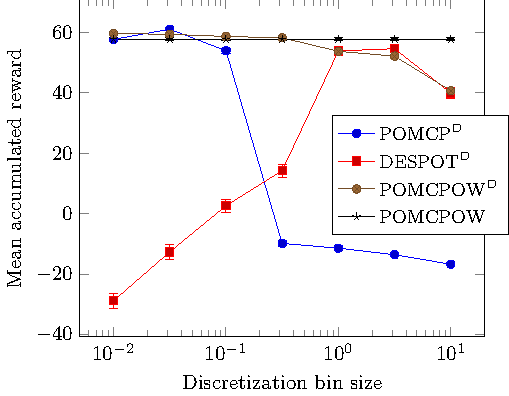
\includegraphics[width=0.8\linewidth]{media/ld_discretization.pdf}
        \caption{Light Dark} \label{fig:lddisc}
    \end{subfigure}

    \begin{subfigure}{\linewidth}
        \centering
        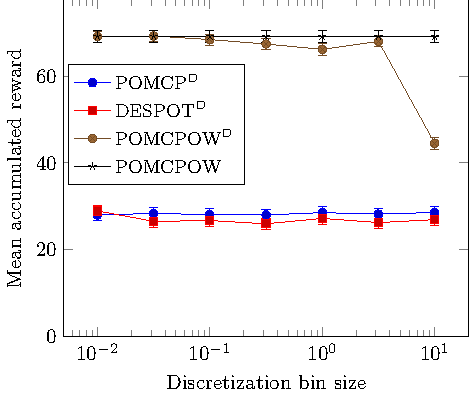
\includegraphics[width=0.72\linewidth]{media/subhunt_discretization.pdf}
        \caption{Sub Hunt}
        \label{fig:shdisc}
    \end{subfigure}

    \caption{Discretization granularity studies} \label{fig:disc}
\end{figure}



\subsection{Observation Distribution Requirement}

It is important to note that, while POMCP, POMCP-DPW, and DESPOT only require a generative model of the problem,  both POMCPOW and PFT-DPW require a way to query the relative likelihood of different observations ($\odist$ in line~\ref{lin:weight}).
One may object that this will limit the application of POMCPOW to a small class of POMDPs, but we think it will be an effective tool in practice for two reasons.

First, this requirement is no more stringent than the requirement for a standard importance resampling particle filter, and such filters are used widely, at least in the field of robotics that the authors are most familiar with. 
Moreover, if the observation model is complex, an approximate model may be sufficient.

Second, given the implications of \cref{thm:qmdp}, it is difficult to imagine a tree-based decision-making algorithm or a robust belief updater that does not require some way of measuring whether a state belongs to a belief or history.
The observation model is a straightforward and standard way of specifying such a measure.
Finally, in practice, except for the simplest of problems, using POMCP or DESPOT to repeatedly observe and act in an environment already requires more than just a generative model.
For example, the authors of the original paper describing POMCP~\cite{silver2010pomcp} use heuristic particle reinvigoration in lieu of an observation model and importance sampling.

\section{Experiments} \label{sec:experiments}

Numerical simulation experiments were conducted to evaluate the performance of POMCPOW and PFT-DPW compared to other solvers. The open source code for the experiments is built on the POMDPs.jl framework \cite{egorov2017pomdps} and is hosted at \url{https://github.com/zsunberg/ContinuousPOMDPTreeSearchExperiments.jl}. In all experiments, the solvers were limited to \SI{1}{second} of computation time per step. Belief updates were accomplished with a particle filter independent of the planner, and no part of the tree was saved for re-use on subsequent steps. Hyperparameter values are shown in \cref{sec:hyper}.

\begin{sidewaystable}
    {
        \caption{Experimental Results} \label{tab:experiments}

        \begin{tabularx}{\linewidth}{lXrlXrlXrl}
\toprule
& & Laser Tag \makebox[0pt][l]{(D, D, D)} & & & Light Dark \makebox[0pt][l]{(D, D, C)} & & & Sub Hunt \makebox[0pt][l]{(D, D, C)} & \\
\midrule
POMCPOW & & \result{-10.3}{0.2}{81}{0.81} & & \result{56.1}{0.6}{76}{0.76} & & \result{69.2}{1.3}{87}{0.87} \\
PFT-DPW & & \result{-11.1}{0.2}{74}{0.74} & & \result{57.2}{0.5}{77}{0.77} & & \result{77.4}{1.1}{97}{0.97} \\
QMDP & & \result{-10.5}{0.2}{79}{0.79} & & \result{-6.4}{1.0}{14}{0.14} & & \result{28.0}{1.3}{35}{0.35} \\
POMCP-DPW & & \result{-10.6}{0.2}{78}{0.78} & & \result{-7.3}{1.0}{13}{0.13} & & \result{28.3}{1.3}{35}{0.35} \\
DESPOT & & \result{-8.9}{0.2}{92}{0.92} & & \result{-6.8}{1.0}{13}{0.13} & & \result{26.8}{1.3}{34}{0.34} \\
POMCP\textsuperscript{D} & & \result{-14.1}{0.2}{49}{0.49} & & \result{61.1}{0.4}{81}{0.81} & & \result{28.0}{1.3}{35}{0.35} \\
DESPOT\textsuperscript{D} & & \noresult{} & & \result{54.2}{1.1}{74}{0.74} & & \result{27.4}{1.3}{34}{0.34} \\

\midrule
& & VDP Tag \makebox[0pt][l]{(C, C, C)} & & & Multilane \makebox[0pt][l]{(C, D, C)} & \\
\midrule
POMCPOW & & \result{29.3}{0.8}{95}{0.95} & & \result{30.9}{0.9}{70}{0.70} \\
PFT-DPW & & \result{27.2}{0.8}{88}{0.88} & & \result{21.4}{0.9}{38}{0.38} \\
QMDP & & \noresult{} & & \noresult{} \\
POMCP-DPW & & \result{16.4}{1.0}{53}{0.53} & & \result{29.6}{0.9}{65}{0.65} \\
DESPOT & & \noresult{} & & \result{36.0}{0.8}{87}{0.87} \\
POMCP\textsuperscript{D} & & \result{14.7}{0.9}{47}{0.47} & & \noresult{} \\
DESPOT\textsuperscript{D} & & \result{14.3}{1.0}{46}{0.46} & & \noresult{} \\

\bottomrule
\end{tabularx}


    }
    \vspace{5mm}
    \footnotesize{The three C or D characters after the solver indicate whether the state, action, and observation spaces are continuous or discrete, respectively. For continuous problems, solvers with a superscript D were run on a version of the problem with discretized action and observation spaces, but they interacted with continuous simulations of the problem.}
\end{sidewaystable}

\subsection{Laser Tag}

The Laser Tag benchmark is taken directly from the work of \citet{somani2013despot} and included for the sake of calibration. DESPOT outperforms the other methods. The score for DESPOT differs slightly from that reported by \citet{somani2013despot} likely because of bounds implementation differences.
POMCP performs much better than reported by \citet{somani2013despot} because this implementation uses a state-based rollout policy.

\subsection{Light Dark}

In the Light Dark domain, the state is an integer, and the agent can choose how to move deterministically ($s' = s+a$) from the action space $\mathcal{A}=\{-10, -1, 0, 1, -10\}$. 
The goal is to reach the origin.
If action $0$ is taken at the origin, a reward of $100$ is given and the problem terminates; If action $0$ is taken at another location, a penalty of $-100$ is given.
There is a cost of $-1$ at each step before termination.
The agent receives a more accurate observation in the ``light'' region around $s=10$.
Specifically, observations are continuous ($\ospace=\reals$) and normally distributed with standard deviation $\sigma=|s-10|$.

\Cref{tab:experiments} shows the mean reward from $1000$ simulations for each solver, and \cref{fig:ld} shows an example experiment.
The optimal strategy involves moving toward the light region and localizing before proceeding to the origin. 
QMDP and solvers predicted to behave like QMDP attempt to move directly to the origin, while POMCPOW and PFT-DPW perform better.
In this one-dimensional case, discretization allows POMCP to outperform all other methods and DESPOT to perform well, but in subsequent problems where the observation space has more dimensions, discretization does not provide the same performance improvement (see \cref{sec:discretization}).

\begin{figure}[htb]
    \centering
    % \input{ld_fig.pgf}
    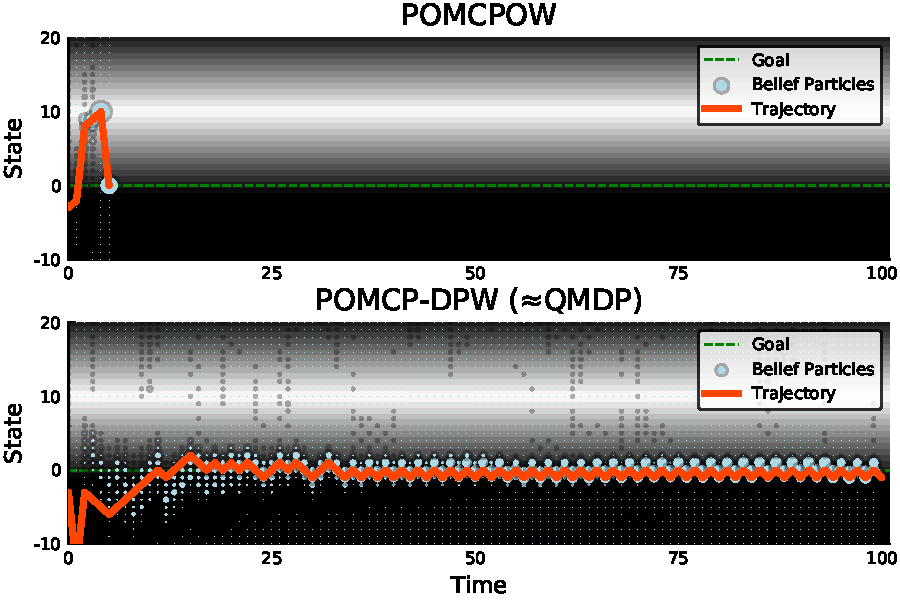
\includegraphics[width=\columnwidth]{media/ld_fig.pdf}
    \caption{Example trajectories in the Light Dark domain. POMCPOW travels to the light region and accurately localizes before moving to the goal. POMCP-DPW displays QMDP-like behavior: it is unable to localize well enough to take action \num{0} with confidence. The belief particles far away from \num{0} in the POMCP-DPW plot are due to particle reinvigoration that makes the filter more robust.}
    \label{fig:ld}
\end{figure}

\subsection{Sub Hunt}

In the Sub Hunt domain, the agent is a submarine attempting to track and destroy an enemy sub.
The state and action spaces are discrete so that QMDP can be used to solve the problem for comparison.
The agent and the target each occupy a cell of a 20 by 20 grid. The target is either aware or unaware of the agent and seeks to reach a particular edge of the grid unknown to the agent ($\mathcal{S} = \{1,..,20\}^4 \times \{\text{aware}, \text{unaware}\} \times \{N,S,E,W\}$).
The target stochastically moves either two steps towards the goal or one step forward and one to the side.
The agent has six actions, move three steps north, south, east, or west, engage the other submarine, or ping with active sonar.
If the agent chooses to engage and the target is unaware and within a range of 2, a hit with reward 100 is scored; The problem ends when a hit is scored or the target reaches its goal edge.

An observation consists of 8 sonar returns ($\ospace = \reals^8$) at equally-spaced angles that give a normally distributed estimate ($\sigma=0.5$) of the range to the target if the target is within that beam and a measurement with higher variance if it is not.
The range of the sensors depends on whether the agent decides to use active sonar.
If the agent does not use active sonar it can only detect the other submarine within a radius of 3, but pinging with active sonar will detect at any range.
However, active sonar alerts the target to the presence of the agent, and when the target is aware, the hit probability when engaging drops to $60\%$.

\Cref{tab:experiments} shows the mean reward for $1000$ simulations for each solver.
The optimal strategy includes using the active sonar, but previous approaches have difficulty determining this because of the reduced engagement success rate.
The PFT-DPW approach has the best score, followed closely by POMCPOW.
All other solvers have similar performance to QMDP.


\subsection{Van Der Pol Tag} \label{sec:vdptag}

\begin{figure}[bth]
    \centering
    \begin{minipage}{0.5\linewidth}
        \centering
        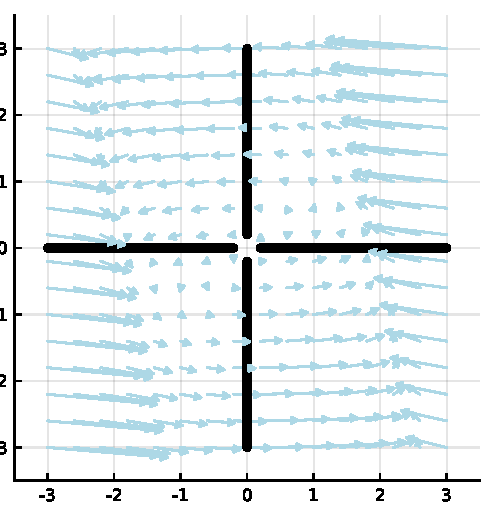
\includegraphics[width=0.8\linewidth]{media/vdp_quiver.pdf}
    \end{minipage}
    \hfill
    \begin{minipage}[c]{0.45\linewidth}
        \caption{Van Der Pol tag problem. The arrows show the target differential equation, and the thick black lines represent the barriers.}
        \label{fig:vdp}
    \end{minipage}
\end{figure}


The final experimental problem is called Van Der Pol tag and has continuous state, action, and observation spaces.
In this problem an agent moves through 2D space to try to tag a target ($\mathcal{S}=\reals^4$) that has a random unknown initial position in $[-4, 4]\times[-4,4]$.
The agent always travels at the same speed, but chooses a direction of travel and whether to take an accurate observation ($\mathcal{A} = [0, 2\pi)\times\{0,1\}$).
The observation again consists of 8 beams ($\ospace=\reals^8$) that give measurements to the target.
Normally, these measurements are too noisy to be useful ($\sigma=5$), but, if the agent chooses an accurate measurement with a cost of \num{5}, the observation has low noise ($\sigma=0.1$).
The agent is blocked if it comes into contact with one of the barriers that stretch from \num{0.2} to \num{3.0} in each of the cardinal directions (see \cref{fig:vdp}), while the target can move freely through.
There is a cost of \num{1} for each step, and a reward of \num{100} for tagging the target (being within a distance of \num{0.1}).


The target moves following a two dimensional form of the Van Der Pol oscillation defined by the differential equations%
\begin{equation}
    \dot{x} = \mu \left( x - \frac{x^3}{3} -y \right) \quad \text{ and }\quad \dot{y} = \frac{1}{\mu}x\text{,} \nonumber
\end{equation}
where $\mu=2$.
Gaussian noise ($\sigma=0.05$) is added to the position at the end of each step.
Runge-Kutta fourth order integration is used to propagate the state.

This problem has several challenging features that might be faced in real-world applications.
First, the state transitions are more computationally expensive because of the numerical integration.
Second, the continuous state space and obstacles make it difficult to construct a good heuristic rollout policy, so random rollouts are used.
\Cref{tab:experiments} shows the mean reward for $1000$ simulations of this problem for each solver.
Since a POMCPOW iteration requires less computation than a PFT-DPW iteration, POMCPOW simulates more random rollouts and thus performs slightly better.

\todo{Add Multilane Section}

\subsection{Hyperparameters} \label{sec:hyper}

\begin{table}[t]
    {\centering
\caption{Hyperparameters used in experiments} \label{tab:hyper}

\begin{center}
\begin{tabular}{lrrrr}
    \toprule
                & Laser Tag     & Light Dark    & Sub Hunt      & VDP Tag \\
    \midrule
    \multicolumn{3}{l}{POMCPOW} \\
    \midrule
    $c$         & \num{26.0}    & \num{90.0}    & \num{17.0}    & \num{110.0} \\
    $k_a$       & --            & --            & --            & \num{30.0}  \\
    $\alpha_a$  & --            & --            & --            & \num{1/30}  \\
    $k_o$       & \num{4.0}     & \num{5.0}     & \num{6.0}     & \num{5.0}   \\
    $\alpha_o$  & \num{1/35}    & \num{1/15}    & \num{1/100}   & \num{1/100} \\
    \midrule
    \multicolumn{3}{l}{PFT-DPW} \\
    \midrule
    $m$         & \num{20}      & \num{20}      & \num{20}      & \num{20}    \\
    $c$         & \num{26.0}    & \num{100.0}   & \num{100.0}   & \num{70.0}  \\
    $k_a$       & --            & --            & --            & \num{20.0}  \\
    $\alpha_a$  & --            & --            & --            & \num{1/25}  \\
    $k_o$       & \num{4.0}     & \num{4.0}     & \num{2.0}     & \num{8.0}   \\
    $\alpha_o$  & \num{1/35}    & \num{1/10}    & \num{1/10}    & \num{1/85}  \\
    \midrule

\end{tabular}
\end{center}
    }
    \vspace{1mm}

    \footnotesize{For problems with discrete actions, all actions are considered and $k_a$ and $\alpha_a$ are not needed.}
\end{table}

Hyperparameters for POMCPOW and PFT-DPW were chosen using the cross entropy method \cite{mannor2003cross}, but exact tuning was not a high priority and some parameters were re-used across solvers so the parameters may not be perfectly optimized.
The values used in the experiments are shown in \cref{tab:hyper}. 
There are not enough experiments to draw broad conclusions about the hyperparameters, but it appears that performance is most sensitive to the exploration constant, $c$.

The values for the observation widening parameters, $k_o$ and $\alpha_o$, were similar for all the problems in this work.
A small $\alpha_o$ essentially limits the number of observations to a static number $k_o$, resulting in behavior reminiscent of sparse UCT \cite{browne2012survey}, preventing unnecessary widening and allowing the tree to grow deep.
This seems to work well in practice with the branching factor ($k_o$) set to values between \num{2} and \num{8}, and suggests that it may be sufficient to limit the number of children to a fixed number rather than do progressive widening in a real implementation.


